\begin{frame}
   \only<1-6>{\frametitle{Talk Outline}}
   \only<7->{\frametitle{Lazily Evaluated Marginal Utility Roadmaps}}
   \begin{tikzpicture}[font=\small]
   \draw[step=1,black!15,very thin,opacity=\gridopacity] (0,0) grid (12,8);
   \tikzset{>=latex} % arrow heads

   % START LEMUR
   \node[fill=blue!5,draw=blue!10,rounded corners,minimum width=9.7cm,minimum height=5.8cm,anchor=north] (lemur) at (6,6.0) {};
   \only<1-6>{\node[anchor=north west] at (lemur.north west) {Planner};}
   \only<7->{\node[anchor=north west] at (lemur.north west) {LEMUR};}

   % left side

   \node[fill=blue!10,draw=blue!20,rounded corners,align=center,minimum height=1.5cm,minimum width=2.5cm,inner sep=0pt] at (3.3,4.5) {};
   \node at (3.3,4.5) {\includegraphics[width=1.8cm]{build/roadmap-stack-short}};
   \draw[->] (3.3,3.75) -- (3.3,3.0) node [pos=0.45,fill=blue!5,align=center,inner sep=2pt] {$G$};

   % right side

   \node[fill=blue!10,draw=blue!20,rounded corners,align=center,minimum height=1.5cm,inner sep=0pt] at (7.8,4.5) {
      \qquad\qquad\; $ \arraycolsep=1.5pt \begin{array}{rcc}
         w_{\ms{est}}(e) = & \lambda \, \grave{p}(e) \; + & (1\!-\!\lambda) \, \hat{x}(e) \\
         w(e) = & & (1\!-\!\lambda) \, x(e)
      \end{array} $
   };
   %\node[fill=black!3,draw=blue!20,inner sep=2pt] at (7,5.4) {\includegraphics[width=1.3cm]{build/pvx-utility-anytime-simple}};
   \node[fill=black!3,draw=blue!20,inner sep=2pt] at (5.6,4.5) {\includegraphics[width=1.0cm]{build/pvx-linear-discounting-simple}};

   \draw[->] (7.3,3.75) -- (7.3,3.0) node [pos=0.45,fill=blue!5,align=center,inner sep=2pt] {$w$};
   \draw[->] (8.2,3.75) -- (8.2,3.0) node [pos=0.45,fill=blue!5,align=center,inner sep=2pt] {$w_{\ms{est}}$};

   % START LAZYSP
   \node[fill=blue!10,draw=blue!20,rounded corners,minimum width=7cm,minimum height=2.5cm,anchor=north] (lazysp) at (6,3.0) {};
   \only<2->{\node[anchor=north west] at (lazysp.north west) {\strut LazySP};}

   \only<3->{
   \node[fill=blue!20,draw=blue!30,rounded corners,align=center,minimum height=1cm] (dynsp) at (4.3,1.7) {DynamicSP};
   }

   \only<4->{
      \draw[->] (dynsp.south) -- (4.3,0.8) -- (7.7,0.8) -- (7.7,1.2);
      \node[fill=blue!10,align=center,inner sep=2pt] at (6,0.8)
         {$\pi_{\ms{candidate}}$};
   }
   
   \only<5->{
      \node[fill=blue!20,draw=blue!30,rounded corners,align=center,minimum height=1cm] (selector) at (7.7,1.7) {Edge Selector\\(e.g. Alternate)};
   }
   
   \only<6->{
      \draw[->] (selector.north) -- (7.7,2.6) -- (4.3,2.6) -- (dynsp.north);
      \node[fill=blue!10,align=center,inner sep=2pt] at (6,2.6)
         {$E_{\ms{changed}}$};
   }

   % END LAZYSP

   % END LEMUR

   % top left side
   \node[fill=blue!10,draw=blue!20,rounded corners,align=center,minimum height=1.5cm,minimum width=1.8cm,inner sep=0pt] at (3.3,7.0) {};
   \node[fill=white,inner sep=0pt] at (3.3,7.0) {\includegraphics[width=1.4cm]{build/c-space-simple}};
   \node[font=\scriptsize] at (2.95,6.7) {$\mathcal{C}_{\mbox{\tiny free}}$};
   \draw[->] (3.3,6.25) -- (3.3,5.25) node [pos=0.55,fill=blue!5,align=center,inner sep=0pt] {\strut $\mathcal{C}$};

   %\node[inner sep=4pt] (cspace) at (3.3,7.0) {$\mathcal{C}$-Space};
   %\draw[->] (cspace) -- (3.3,5.25);
   
   % top right side
   \node[fill=blue!10,draw=blue!20,rounded corners,align=center,minimum height=1.5cm] at (7.9,7)
   {$\arraycolsep=1.5pt \begin{array}{cl}
      x(\xi)\!: & \mbox{execution cost} \;(\mathcal{C}_{\ms{free}}) \\
      \hat{x}(\xi)\!: & \mbox{execution cost estimate} \\
      \grave{p}(\xi)\!: & \mbox{planning cost estimate}
   \end{array}$};
   
   \draw[->] (7.3,6.25) -- (7.3,5.25) node [pos=0.55,fill=blue!5,align=center,inner sep=0pt] {\strut $x$};
   \draw[->] (7.9,6.25) -- (7.9,5.25) node [pos=0.55,fill=blue!5,align=center,inner sep=0pt] {\strut $\hat{x}$};
   \draw[->] (8.5,6.25) -- (8.5,5.25) node [pos=0.55,fill=blue!5,align=center,inner sep=0pt] {\strut $\grave{p}$};

   % left side
   \draw[->] (0.5,2.0) -- (2.5,2.0);
   \node[fill=white,align=center,inner sep=2pt] at (0.5,2.0)
      {$q_{\ms{start}}$\\$q_{\ms{dest}}$};

   % right side
   \draw[->] (9.5,2.0) -- (11.3,2.0);
   \node[fill=white,align=center,inner sep=2pt] at (11.5,2.0)
      {$\xi$};

   \end{tikzpicture}
\end{frame}


\begin{frame}
   \frametitle{Lazy SP: The Inner DynamicSP Search}
   \begin{tikzpicture}[font=\small]
      \draw[step=1,black!15,very thin,opacity=\gridopacity] (0,0) grid (12,8);
      
      %% graph start
      %\coordinate (va) at ( 2.0,5.6);
      %\coordinate (vb) at ( 3.5,6.3);
      %\coordinate (vc) at ( 4.0,7.5);
      %\coordinate (vd) at ( 5.5,6.1);
      %\coordinate (ve) at ( 8.0,6.6);
      %\coordinate (vf) at (10.0,5.6);
      %\coordinate (vg) at ( 1.5,6.6);
      %\coordinate (vh) at ( 4.0,5.1);
      %\coordinate (vi) at ( 7.0,4.8);
      %\coordinate (vj) at ( 6.5,7.1);
      %\coordinate (vk) at ( 9.0,5.1);
      %
      %% start/goal highlighting
      %\node[circle,fill=black!20,inner sep=0.1cm] at (va) {};
      %\node[circle,fill=black!20,inner sep=0.1cm] at (vf) {};
      %
      %% candidate paths
      %\draw[line width=0.2cm,color=black!30,line cap=round]
      %   (va) -- (vb) -- (vd) -- (vj) -- (ve) -- (vf);
      %\draw[line width=0.2cm,color=blue!70,line cap=round]
      %   (vj) -- (ve);
      %
      %\draw[black!30] (va) -- (vb) node[midway,circle,inner sep=0.02cm,fill=white,opacity=0.9,font=\scriptsize] {5?};
      %\draw[black!30] (vb) -- (vd) node[midway,circle,inner sep=0.02cm,fill=white,opacity=0.9,font=\scriptsize] {6?};
      %\draw[black!30] (va) -- (vh) node[midway,circle,inner sep=0.02cm,fill=white,opacity=0.9,font=\scriptsize] {6?};
      %\draw[black!30] (vh) -- (vd) node[midway,circle,inner sep=0.02cm,fill=white,opacity=0.9,font=\scriptsize] {7?};
      %\draw[black!30] (vb) -- (vc) node[midway,circle,inner sep=0.02cm,fill=white,opacity=0.9,font=\scriptsize] {5?};
      %\draw[black!30] (vc) -- (vj) node[midway,circle,inner sep=0.02cm,fill=white,opacity=0.9,font=\scriptsize] {8?};
      %\draw[black!30] (va) -- (vg) node[midway,circle,inner sep=0.02cm,fill=white,opacity=0.9,font=\scriptsize] {3?};
      %\draw[black!30] (vb) -- (vg) node[midway,circle,inner sep=0.02cm,fill=white,opacity=0.9,font=\scriptsize] {6?};
      %\draw[black!30] (vb) -- (vh) node[midway,circle,inner sep=0.02cm,fill=white,opacity=0.9,font=\scriptsize] {5?};
      %\draw[black!30] (vc) -- (vd) node[midway,circle,inner sep=0.02cm,fill=white,opacity=0.9,font=\scriptsize] {7?};
      %\draw[black!30] (ve) -- (vf) node[midway,circle,inner sep=0.02cm,fill=white,opacity=0.9,font=\scriptsize] {7?};
      %\draw[black!30] (vd) -- (vi) node[midway,circle,inner sep=0.02cm,fill=white,opacity=0.9,font=\scriptsize] {8?};
      %\draw[black!30] (ve) -- (vi) node[midway,circle,inner sep=0.02cm,fill=white,opacity=0.9,font=\scriptsize] {8?};
      %\draw[black!30] (vd) -- (vj) node[midway,circle,inner sep=0.02cm,fill=white,opacity=0.9,font=\scriptsize] {6?};
      %\draw[black!30] (vf) -- (vk) node[midway,circle,inner sep=0.02cm,fill=white,opacity=0.9,font=\scriptsize] {3?};
      %\draw[black!30] (vi) -- (vk) node[midway,circle,inner sep=0.02cm,fill=white,opacity=0.9,font=\scriptsize] {6?};
      %\draw[black!30] (ve) -- (vk) node[midway,circle,inner sep=0.02cm,fill=white,opacity=0.9,font=\scriptsize] {6?};
      %
      %\draw[black,ultra thick] (vd) -- (ve) node[midway,circle,inner sep=0.02cm,fill=white,opacity=0.9,font=\scriptsize] {$\infty$};
      %\draw[black!30] (ve) -- (vj) node[midway,circle,inner sep=0.02cm,fill=white,opacity=0.9,font=\scriptsize] {4?};
      %
      %\node[circle,fill=black,inner sep=0.05cm] at (va) {};
      %\node[circle,fill=black,inner sep=0.05cm] at (vb) {};
      %\node[circle,fill=black,inner sep=0.05cm] at (vc) {};
      %\node[circle,fill=black,inner sep=0.05cm] at (vd) {};
      %\node[circle,fill=black,inner sep=0.05cm] at (ve) {};
      %\node[circle,fill=black,inner sep=0.05cm] at (vf) {};
      %\node[circle,fill=black,inner sep=0.05cm] at (vg) {};
      %\node[circle,fill=black,inner sep=0.05cm] at (vh) {};
      %\node[circle,fill=black,inner sep=0.05cm] at (vi) {};
      %\node[circle,fill=black,inner sep=0.05cm] at (vj) {};
      %\node[circle,fill=black,inner sep=0.05cm] at (vk) {};
      %
      %\node[left=0.1cm of va] {$v_s$};
      %\node[right=0.1cm of vf] {$v_t$};
      % graph end
      
      % here's an algorithm
      
      \node[inner sep=0.2cm,fill=blue!10,rounded corners,anchor=north,minimum height=4.3cm,minimum width=7.5cm] at (6,7.75) {};
      \only<2>{
         \node[inner sep=0.2cm,fill=blue!30,anchor=north,minimum height=0.5cm,minimum width=7.5cm] at (6,6.15) {};
      }
      \node[inner sep=0.0cm,anchor=north] at (6,7.65)
      {\hspace*{-0.6cm}\begin{minipage}{7.5cm}\small{
      \algrenewcommand{\alglinenumber}[1]{}
      \begin{algorithmic}[1]
         \Function {\textsc{LazySP}}{$G, v_s, v_g, w, w_{\ms{est}}$}
         \State $E_{\ms{eval}} \leftarrow \emptyset$
         \State $w_{\ms{lazy}}(e) \leftarrow w_{\ms{est}}(e) \quad \forall e \in E$
         \Loop
            \vspace{0.05cm}
            \State $p_{\ms{candidate}} \leftarrow
               \mbox{\sc DynamicSP}(G, v_s, v_g, w_{\ms{lazy}})$ %\Comment Compute the shortest path with lazy edge weights
            \vspace{0.1cm}
            %\vspace{0.2cm}
            %\If {$p_{\ms{candidate}} \subseteq E_{\ms{eval}}$} \Comment If path is fully evaluated,
            %   \State \Return $p_{\ms{candidate}}$ \Comment return it
            %\EndIf
            \State \textbf{if} $p_{\ms{candidate}} \subseteq E_{\ms{eval}}$ \textbf{then return} $p_{\ms{candidate}}$
            \vspace{0.1cm}
            \State $E_{\ms{selected}} \leftarrow  \mbox{\sc EdgeSelector}(G, p_{\ms{candidate}})$ %\Comment Select edges on path to process
            \For {$e \in E_{\ms{selected}} \setminus E_{\ms{eval}}$} %\Comment For all unevaluated selected edges
               \State $w_{\ms{lazy}}(e) \leftarrow w(e)$
               \State $E_{\ms{eval}} \leftarrow E_{\ms{eval}} \cup e$ %\Comment Add to evaluated edge set
            \EndFor
         \EndLoop
         \EndFunction
      \end{algorithmic}
      }\end{minipage}};


      \node[fill=blue!10,draw=blue!20,rounded corners,align=center,minimum height=1.8cm,inner sep=2pt,anchor=north] at (3.0,3.0) {
         Motion Planning:\\
         \vspace{-0.3cm}\\
         $ \arraycolsep=1.5pt \def\arraystretch{1.5} \begin{array}{rl}
            {\hat x}(e) = & ||e|| \\
            x(e) = & \left\{ \arraycolsep=2pt \def\arraystretch{1.0} \begin{array}{cl}
               ||e|| & e \in C_{\ms{free}} \\
               \infty & \mbox{otherwise}
               \end{array} \right. \\
            h_x(v) = & || v - v_g ||
         \end{array} $
      };
      

      \node[fill=blue!10,draw=blue!20,rounded corners,align=center,minimum height=1.8cm,inner sep=2pt,anchor=north] at (8.6,3.0) {
         Maximizing Utility:\\
         \vspace{-0.3cm}\\
         \qquad\qquad\; $ \arraycolsep=1.5pt \def\arraystretch{1.2} \begin{array}{rcl}
            w_{\ms{est}}(e) = & \lambda \, \grave{p}(e) \; + & (1\!-\!\lambda) \, \hat{x}(e) \\
            w(e) = & & (1\!-\!\lambda) \, x(e) \\
            h_w(v) = & & (1\!-\!\lambda) \, h_x(v)
         \end{array} $
      };
      \node[fill=black!3,draw=blue!20,inner sep=2pt] at (6.35,1.85) {\includegraphics[width=1.0cm]{build/pvx-linear-discounting-simple}};
         
      
   %Augment problem with inexpensive edge heuristic. (Show augmentation.)
   %Each edge has binary state.
   
   %Show outline of algorithm.
   
   %Two core sub-routines: inner SP search, and edge selector.
   \end{tikzpicture}
\end{frame}

\begin{frame}
   \frametitle{LazySP: DynamicSP Algorithms}
   \begin{tikzpicture}[font=\small]
      \draw[step=1,black!15,very thin,opacity=\gridopacity] (0,0) grid (12,8);

      \node at (6,4) {\includegraphics{build/ibid-lazysp-plot,hideibid}};

      %\node[draw=black!30,inner sep=0pt] at (3.5,5.0) {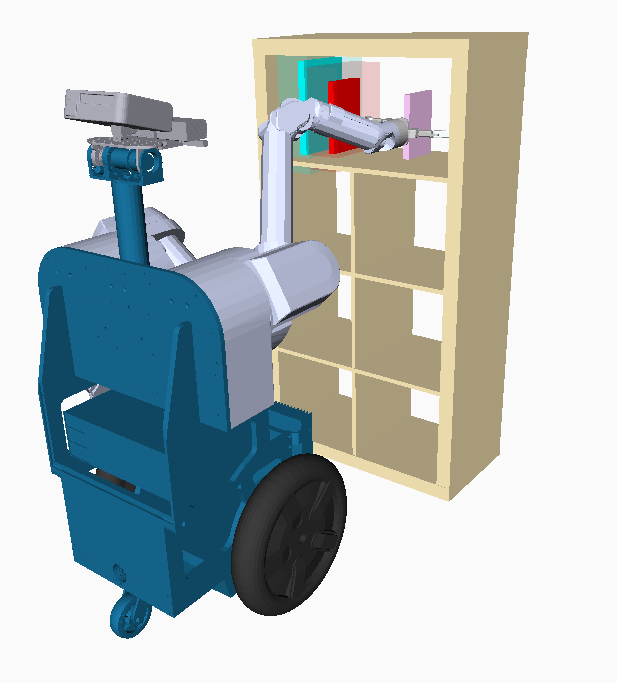
\includegraphics[width=2.5cm]{figs/herbarm-traj2-t031.png}};
      \node[draw=black,inner sep=0pt,thick,anchor=north] at (5.15,7.325) {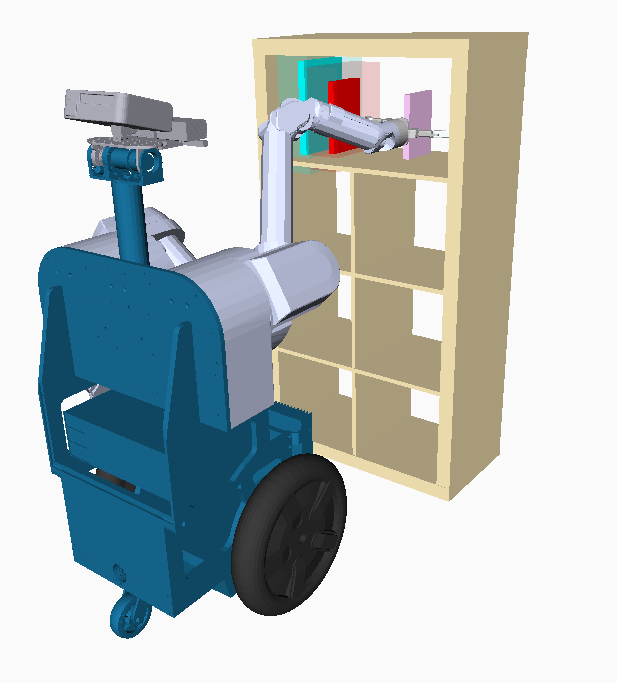
\includegraphics[width=2.0cm]{figs/herbarm-traj2-t031.png}};
      \node[draw=black,fill=black!2,anchor=north] at (7.8,7.325) {\strut $h_w = (1 - \lambda) \, h_x$};

   \end{tikzpicture}
\end{frame}

\begin{frame}
   \frametitle{Talk Outline}
   \begin{tikzpicture}[font=\small]
   \draw[step=1,black!15,very thin,opacity=\gridopacity] (0,0) grid (12,8);
   \tikzset{>=latex} % arrow heads

   % START LEMUR
   \node[fill=blue!5,draw=blue!10,rounded corners,minimum width=9.7cm,minimum height=5.8cm,anchor=north] (lemur) at (6,6.0) {};
   \node[anchor=north west] at (lemur.north west) {LEMUR};

   % left side

   \node[fill=blue!10,draw=blue!20,rounded corners,align=center,minimum height=1.5cm,minimum width=2.5cm,inner sep=0pt] at (3.3,4.5) {};
   \node at (3.3,4.5) {\includegraphics[width=1.8cm]{build/roadmap-stack-short}};
   \draw[->] (3.3,3.75) -- (3.3,3.0) node [pos=0.45,fill=blue!5,align=center,inner sep=2pt] {$G$};

   % right side

   \node[fill=blue!10,draw=blue!20,rounded corners,align=center,minimum height=1.5cm,inner sep=0pt] at (7.8,4.5) {
      \qquad\qquad\; $ \arraycolsep=1.5pt \begin{array}{rcc}
         w_{\ms{est}}(e) = & \lambda \, \grave{p}(e) \; + & (1\!-\!\lambda) \, \hat{x}(e) \\
         w(e) = & & (1\!-\!\lambda) \, x(e)
      \end{array} $
   };
   %\node[fill=black!3,draw=blue!20,inner sep=2pt] at (7,5.4) {\includegraphics[width=1.3cm]{build/pvx-utility-anytime-simple}};
   \node[fill=black!3,draw=blue!20,inner sep=2pt] at (5.6,4.5) {\includegraphics[width=1.0cm]{build/pvx-linear-discounting-simple}};

   \draw[->] (7.3,3.75) -- (7.3,3.0) node [pos=0.45,fill=blue!5,align=center,inner sep=2pt] {$w$};
   \draw[->] (8.2,3.75) -- (8.2,3.0) node [pos=0.45,fill=blue!5,align=center,inner sep=2pt] {$w_{\ms{est}}$};

   % START LAZYSP
   \node[fill=blue!10,draw=blue!20,rounded corners,minimum width=7cm,minimum height=2.5cm,anchor=north] (lazysp) at (6,3.0) {};
   \node[anchor=north west] at (lazysp.north west) {\strut LazySP};

   \node[fill=blue!20,draw=blue!30,rounded corners,align=center,minimum height=1cm] (dynsp) at (4.3,1.7) {DynamicSP};

   \draw[->] (dynsp.south) -- (4.3,0.8) -- (7.7,0.8) -- (7.7,1.2);
   \node[fill=blue!10,align=center,inner sep=2pt] at (6,0.8)
      {$\pi_{\ms{candidate}}$};

   \node[fill=blue!20,draw=blue!30,rounded corners,align=center,minimum height=1cm] (selector) at (7.7,1.7) {Edge Selector\\(e.g. Alternate)};

   \draw[->] (selector.north) -- (7.7,2.6) -- (4.3,2.6) -- (dynsp.north);
   \node[fill=blue!10,align=center,inner sep=2pt] at (6,2.6)
      {$E_{\ms{changed}}$};

   % END LAZYSP

   % END LEMUR

   % top left side
   \node[fill=blue!10,draw=blue!20,rounded corners,align=center,minimum height=1.5cm,minimum width=1.8cm,inner sep=0pt] at (3.3,7.0) {};
   \node[fill=white,inner sep=0pt] at (3.3,7.0) {\includegraphics[width=1.4cm]{build/c-space-simple}};
   \node[font=\scriptsize] at (2.95,6.7) {$\mathcal{C}_{\mbox{\tiny free}}$};
   \draw[->] (3.3,6.25) -- (3.3,5.25) node [pos=0.55,fill=blue!5,align=center,inner sep=0pt] {\strut $\mathcal{C}$};

   %\node[inner sep=4pt] (cspace) at (3.3,7.0) {$\mathcal{C}$-Space};
   %\draw[->] (cspace) -- (3.3,5.25);
   
   % top right side
   \node[fill=blue!10,draw=blue!20,rounded corners,align=center,minimum height=1.5cm] at (7.9,7)
   {$\arraycolsep=1.5pt \begin{array}{cl}
      x(\xi)\!: & \mbox{execution cost} \;(\mathcal{C}_{\ms{free}}) \\
      \hat{x}(\xi)\!: & \mbox{execution cost estimate} \\
      \grave{p}(\xi)\!: & \mbox{planning cost estimate}
   \end{array}$};
   
   \draw[->] (7.3,6.25) -- (7.3,5.25) node [pos=0.55,fill=blue!5,align=center,inner sep=0pt] {\strut $x$};
   \draw[->] (7.9,6.25) -- (7.9,5.25) node [pos=0.55,fill=blue!5,align=center,inner sep=0pt] {\strut $\hat{x}$};
   \draw[->] (8.5,6.25) -- (8.5,5.25) node [pos=0.55,fill=blue!5,align=center,inner sep=0pt] {\strut $\grave{p}$};

   % left side
   \draw[->] (0.5,2.0) -- (2.5,2.0);
   \node[fill=white,align=center,inner sep=2pt] at (0.5,2.0)
      {$q_{\ms{start}}$\\$q_{\ms{dest}}$};

   % right side
   \draw[->] (9.5,2.0) -- (11.3,2.0);
   \node[fill=white,align=center,inner sep=2pt] at (11.5,2.0)
      {$\xi$};

   \only<2->{
      \draw[thick,rounded corners] (dynsp.south west) rectangle (dynsp.north east);
   }

   \end{tikzpicture}
\end{frame}

\begin{frame}
   \frametitle{Approaches for Fast Pathfinding}
   \begin{tikzpicture}[font=\small]
      \tikzset{>=latex} % arrow heads
      \draw[step=1,black!15,very thin,opacity=\gridopacity] (0,0) grid (12,8);

      \node[fill=blue!10,minimum width=7cm,minimum height=2.67361cm,align=center] at (4,5.95) {
         Problem:\\
         Dynamic Single-Pair Shortest Path (SPSP)\\
      };

      \begin{scope}[shift={(8.0,4.6)}]
         \node[inner sep=0pt,anchor=south west] {%
            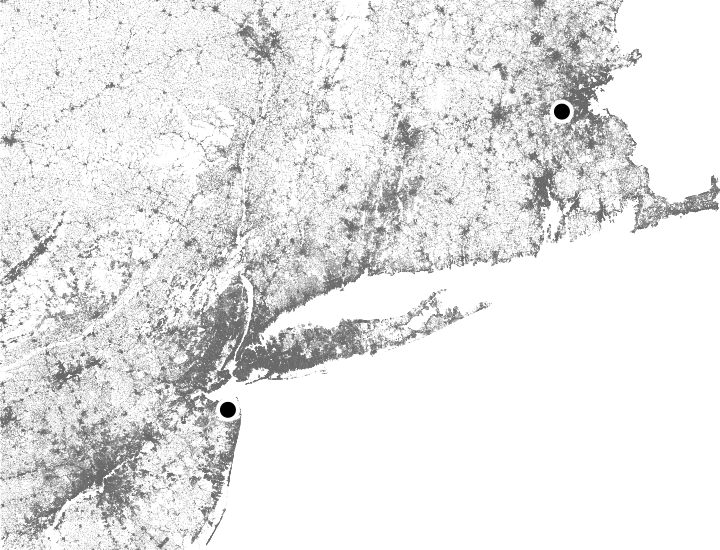
\includegraphics[width=3.5cm]{figs/incbi-road-ne/singleshot/example-intro.png}};
         \coordinate (s) at (1.226,0.63);
         \coordinate (t) at (2.751,1.96);
         \node (slab) at (1.75,0.42) {$s$};
         \node (tlab) at (2.8,1.05) {$t$};
         \draw[->,thick] (slab) -- (s);
         \draw[->,thick] (tlab) -- (t);
      \end{scope}

      \only<2->{
         \node at (2,2.5) {\includegraphics[width=3.5cm]{build/ibid-intro-focus-incremental}};
         \node at (2,3.8) {Incremental Search};
      }

      \only<3->{
         \node at (6,2.5) {\includegraphics[width=3.5cm]{build/ibid-intro-focus-bidirectional}};
         \node at (6,3.8) {Bidirectional Search};
      }

      \only<4->{
         \node at (10,2.5) {\includegraphics[width=3.5cm]{build/ibid-intro-focus-heuristic}};
         \node at (10,3.8) {Heuristic Search};
      }
   
   \end{tikzpicture}
\end{frame}

\begin{frame}
   \frametitle{Outline of Selected Algorithms}
   \begin{tikzpicture}[font=\small]
      \tikzset{>=latex} % arrow heads
      \draw[step=1,black!15,very thin,opacity=\gridopacity] (0,0) grid (12,8);

      %\node at (2,6.3) {\includegraphics[width=3.5cm]{build/ibid-intro-focus-incremental}};
      %\node at (2,7.6) {Incremental Search};

      %\node at (6,6.3) {\includegraphics[width=3.5cm]{build/ibid-intro-focus-bidirectional}};
      %\node at (6,7.6) {Bidirectional Search};

      %\node at (10,6.3) {\includegraphics[width=3.5cm]{build/ibid-intro-focus-heuristic}};
      %\node at (10,7.6) {Heuristic Search};
      

      \only<2->{
      \node[inner sep=0pt,anchor=north] at (6,7.0) {\begin{minipage}{9.05cm}
         \begin{tabular}{ccc}
            \toprule
            & Non-Incremental & {\only<-4>{\color{white}}Incremental} \\
            \midrule
            \addlinespace[0.2em]
            \strut {\only<-2>{\color{white}}Unidirectional}
               & {\only<-2>{\color{white}}Dijkstra's Algorithm}
               & {\only<-4>{\color{white}}DynamicSWSF-FP} \\
            \addlinespace[-0.2em]
            \strut {\only<-3>{\color{white}}\only<12->{\color{gray}}\emph{(Heuristic)}}
               & {\only<-3>{\color{white}}\only<12->{\color{gray}}\emph{A*}}
               & {\only<-4>{\color{white}}\only<12->{\color{gray}}\emph{Lifelong Planning A*}} \\
            \addlinespace[0.3em]
            \strut {\only<-5>{\color{white}}\only<12->{\color{gray}}Bidirectional}
               & {\only<-5>{\color{white}}\only<12->{\color{gray}}Bidirectional Dijkstra}
               & \multirow{2}{*}{\large\only<-6>{\color{white}}\only<9-10>{\color{gray}}?} \\
            \addlinespace[-0.2em]
            \strut {\only<-5>{\color{white}}\only<12->{\color{gray}}\emph{(Heuristic)}}
               & {\only<-5>{\color{white}}\only<12->{\color{gray}}\emph{Bidirectional A*}}
               & \\
            \addlinespace[0.2em]
            \bottomrule
         \end{tabular}
      \end{minipage}};
      }

      \only<8->{
      \node[fill=blue!5,draw=blue!15,rounded corners] at (6,4) {\begin{minipage}{10cm}Key Insights:\end{minipage}};
      }
      
      \only<9->{
         \node[fill=black!5,draw=black!15,rounded corners,
            anchor=north,minimum width=3.0cm,minimum height=2.5cm] (trustblock) at (2.5,3.6) {};
         \node[fill=white,rounded corners,inner sep=2pt,below=0.1cm of trustblock.north]
            {\includegraphics[height=1.7cm]{build/ibid-dijkstra-trust-build,winctrust}};
         \node[align=center,font=\footnotesize,anchor=south] at (trustblock.south) {Trust Regions};
      }
      \only<10->{
         \node[fill=black!5,draw=black!15,rounded corners,
            anchor=north,minimum width=3.0cm,minimum height=2.5cm] (termblock) at (6.0,3.6) {};
         \node[fill=white,rounded corners,inner sep=2pt,below=0.1cm of termblock.north]
            {\includegraphics[height=1.5cm]{build/ibid-bidijkstra-viz-build,e}};
         \node[align=center,font=\footnotesize,anchor=south] at (termblock.south) {Bidirectional\\Termination};
      }
      \only<11->{
         \node[fill=black!5,draw=black!15,rounded corners,
            anchor=north,minimum width=3.0cm,minimum height=2.5cm] (potblock) at (9.5,3.6) {};
         \node[fill=white,rounded corners,inner sep=2pt,below=0.1cm of potblock.north]
            {\includegraphics[height=1.5cm]{build/ibid-potentials}};
         \node[align=center,font=\footnotesize,anchor=south] at (potblock.south) {Potential\\Functions};
      }

      \only<12>{
         \draw[thick,rounded corners] (trustblock.south west) rectangle (trustblock.north east);
      }

      %\only<8-10>{
      %\node[inner sep=0pt,anchor=north] at (6,2.3) {\begin{minipage}{10.9cm}
      %   {\bf 3 Key Insights:}
      %   \begin{itemize}
      %   \item {\only<8-9>{\color{gray}}
      %      Non-Incremental and Incremental methods both create \emph{trust regions (TRs)}}
      %   \item {\color{gray}
      %      Bidirectional termination can be rewritten w.r.t. edges between TRs}
      %   \item {\color{gray}
      %      Heuristic search is equivalent to search over a transformed graph}
      %   \end{itemize}
      %\end{minipage}};
      %}

   \end{tikzpicture}
\end{frame}

\begin{frame}
   \frametitle{Distance Function Approximations \& Trust Regions}
   \begin{tikzpicture}[font=\small]
   \tikzset{>=latex} % arrow heads
   \draw[step=1,black!15,very thin,opacity=\gridopacity] (0,0) grid (12,8);

      % top
      \only<17->{
         \node[fill=black!5,minimum width=5.75cm] at (3,7.5) {\strut Non-Incremental Search};
      }
      \only<18->{
         \node[fill=black!5,minimum width=5.75cm] at (9,7.5) {\strut Incremental Search};
      }

      % middle

      \only<1-18>{
         \node[circle,align=center,fill=green!10,draw=green!50!black,inner sep=0pt,minimum width=0.5cm] (wa) at (6.0,6.8) {$w$};
         \only<2->{
            \node[circle,fill=blue!10,draw=blue!20,densely dashed,inner sep=0pt,minimum width=0.6cm] (dstara) at (6.0,6.0) {\strut $d^*$};
            \draw[->] (wa) -- (dstara);
         }
      }
      \only<19->{
         \node[circle,align=center,fill=green!10,draw=green!50!black,inner sep=0pt,minimum width=0.5cm] (wa) at (6.0,6.8) {$w_a$};
         \node[circle,fill=blue!10,draw=blue!20,densely dashed,inner sep=0pt,minimum width=0.6cm] (dstar1) at (6.0,6.0) {\strut $d^*_a$};
         \draw[->] (wa) -- (dstara);
      }
      \only<20->{
         \node[circle,align=center,fill=green!10,draw=green!50!black,inner sep=0pt,minimum width=0.5cm] (wb) at (6.0,4.8) {$w_b$};
         \node[circle,fill=blue!10,draw=blue!20,densely dashed,inner sep=0pt,minimum width=0.6cm] (dstarb) at (6.0,4.0) {\strut $d^*_b$};
         \draw[->] (wb) -- (dstarb);
      }

      % left side
      \only<3->{
         \node[circle,fill=blue!10,draw=blue!20,inner sep=0pt,minimum width=0.6cm] (ld1) at (2.5,6.0) {\strut $d_1$};
      }

      \only<4->{
         \node[align=center,fill=green!10,draw=green!50!black,rounded corners,anchor=west] (er) at (3.2,5.5) {\strut Edge\\\strut Relaxation};
         \node[circle,fill=green,draw=green!50!black,inner sep=1.5pt] at (er.west) {};
      }

      \only<5->{
         \draw[->] (wa) -- (4.0,6.8) -- (4.0,6.0);
      }

      \only<6->{
         \node[circle,fill=blue!10,draw=blue!20,inner sep=0pt,minimum width=0.6cm] (ld2) at (2.5,5.0) {\strut $d_2$};
         \draw[->] (ld1) .. controls (3.0,5.6) and (3.0,5.4) .. (ld2) node [midway,circle,fill=green,draw=green!50!black,inner sep=1.5pt] {};
      }

      \only<13->{
         \node[fill=black!5,draw=black!15,rounded corners,align=center,
            anchor=north,minimum width=4.8cm,minimum height=3cm] (lefttrustblock) at (2.5,3.6) {};
      }
      \only<14->{
         \node[anchor=north west] at (lefttrustblock.north west) {$d \geq d^*$};
      }
      \only<15->{
         \node[anchor=north east] at (lefttrustblock.north east) {$w \geq 0$};
      }
      \only<16->{
         \node[anchor=south,align=center,font=\footnotesize] at (lefttrustblock.south)
         {If $D$ is the minimal $d(u)$ among\\
            tensioned edges $e_{uv}$, then any\\
            $v$ with $d(v) \leq D$ has $d\!=\!d^*$.};
         \node[fill=white,rounded corners,inner sep=2pt,below=0.1cm of lefttrustblock.north] {\includegraphics[width=2.0cm]{build/ibid-dijkstra-trust-build,wtrust}};
      }

      \only<7->{
         \node[circle,fill=blue!10,draw=blue!20,inner sep=0pt,minimum width=0.6cm] (ld3) at (2.5,4.0) {\strut $d_3$};
         \draw[->] (ld2) .. controls (3.0,4.6) and (3.0,4.4) .. (ld3) node [midway,circle,fill=green,draw=green!50!black,inner sep=1.5pt] {};
      }

      \only<8-11>{
         \begin{scope}
            \clip (1,3.5) rectangle (4,4.5);
            \node[circle,fill=blue!10,draw=blue!20,inner sep=0pt,minimum width=0.6cm] (ld4) at (2.5,3.0) {\strut $d_3$};
            \draw[->] (ld3) .. controls (3.0,3.6) and (3.0,3.4) .. (ld4) node [midway,circle,fill=green,draw=green!50!black,inner sep=1.5pt] {};
         \end{scope}
      }

      \only<9-11>{
         \node[circle,fill=blue!10,draw=blue!20,inner sep=0pt,minimum width=0.6cm] (ldn) at (2.5,2.5) {\strut $d_n$};
         \begin{scope}
            \clip (1,2.0) rectangle (4,3.0);
            \node[circle,fill=blue!10,draw=blue!20,inner sep=0pt,minimum width=0.6cm] (ldnm1) at (2.5,3.5) {\strut $d_{n-1}$};
            \draw[->] (ldnm1) .. controls (3.0,3.1) and (3.0,2.9) .. (ldn) node [midway,circle,fill=green,draw=green!50!black,inner sep=1.5pt] {};
         \end{scope}
      }

      \only<10->{
         \node[align=center,fill=black!5,draw=black!10,rounded corners] (ifd) at (1.0,6.0) {$d \geq d^*$};
      }

      \only<11>{
         \node[align=center,fill=black!5,draw=black!10,rounded corners] (thend) at (1.0,2.5) {then $d_n\!=\!d^*$};
         \draw[->] (ifd) -- (thend);
      }

      \only<21->{
         \node[align=center,fill=red!30,draw=red!50!black,rounded corners] (ifd) at (1.0,4.0) {$d \ngeq d^*$};
      }

      \only<22->{
         \fill[white,opacity=0.5] (0,0.5) rectangle (5,3.6);
      }



      % right side

      \only<23->{
         \node[circle,fill=blue!10,draw=blue!20,inner sep=0pt,minimum width=0.6cm] (rd1) at (9.5,6.0) {\strut $d_1$};
      }

      \only<24->
      {
         \node[align=center,fill=green!10,draw=green!50!black,rounded corners,anchor=east] (vc) at (8.8,5.5) {\strut Vertex\\\strut  Consistency};
         \node[circle,fill=green,draw=green!50!black,inner sep=1.5pt] at (vc.east) {};
      }

      \only<25->{
         \draw[->] (wa) -- (8.0,6.8) -- (8.0,6.0);
      }

      \only<26->{
         \node[circle,fill=blue!10,draw=blue!20,inner sep=0pt,minimum width=0.6cm] (rd2) at (9.5,5.0) {\strut $d_2$};
         \draw[->] (rd1) .. controls (9.0,5.6) and (9.0,5.4) .. (rd2) node [midway,circle,fill=green,draw=green!50!black,inner sep=1.5pt] {};
      }

      \only<27->{
         \node[circle,fill=blue!10,draw=blue!20,inner sep=0pt,minimum width=0.6cm] (rd3) at (9.5,4.0) {\strut $d_3$};
         \draw[->] (rd2) .. controls (9.0,4.6) and (9.0,4.4) .. (rd3) node [midway,circle,fill=green,draw=green!50!black,inner sep=1.5pt] {};
      }

      \only<28->{
         \node[fill=black!5,draw=black!15,rounded corners,
            anchor=north,minimum width=4.8cm,minimum height=3cm] (righttrustblock) at (9.5,3.6) {};
         \node[align=center,font=\footnotesize,anchor=south] at (righttrustblock.south)
         {If $K$ is the minimal
            $k\!=\!\min(d,\!r)$ \\
            among $V_{\ms{\tiny incons}}$, then any consistent \\
            $v$ with $d(v) \leq K$ has $d\!=\!d^*$.};
         \node[anchor=north west] at (righttrustblock.north west) {$w > 0$};
         \node[anchor=north east,color=black!15] at (righttrustblock.north east) {$d \geq d^*$};
         \node[fill=white,rounded corners,inner sep=2pt,below=0.1cm of righttrustblock.north] {\includegraphics[width=2.0cm]{build/ibid-dijkstra-trust-build,winctrust}};
      }

   \end{tikzpicture}
\end{frame}

\begin{frame}
   \frametitle{Outline of Selected Algorithms}
   \begin{tikzpicture}[font=\small]
      \tikzset{>=latex} % arrow heads
      \draw[step=1,black!15,very thin,opacity=\gridopacity] (0,0) grid (12,8);

      \node[inner sep=0pt,anchor=north] at (6,7.0) {\begin{minipage}{9.05cm}
         \begin{tabular}{ccc}
            \toprule
            & Non-Incremental & Incremental \\
            \midrule
            \addlinespace[0.2em]
            \strut Unidirectional
               & Dijkstra's Algorithm
               & DynamicSWSF-FP \\
            \addlinespace[-0.2em]
            \strut {\color{gray}\emph{(Heuristic)}}
               & {\color{gray}\emph{A*}}
               & {\color{gray}\emph{Lifelong Planning A*}} \\
            \addlinespace[0.3em]
            \strut {\only<1>{\color{gray}}Bidirectional}
               & {\only<1>{\color{gray}}Bidirectional Dijkstra}
               & \multirow{2}{*}{\large\color{gray}?} \\
            \addlinespace[-0.2em]
            \strut {\color{gray}\emph{(Heuristic)}}
               & {\color{gray}\emph{Bidirectional A*}}
               & \\
            \addlinespace[0.2em]
            \bottomrule
         \end{tabular}
      \end{minipage}};

      \node[fill=blue!5,draw=blue!15,rounded corners] at (6,4) {\begin{minipage}{10cm}Key Insights:\end{minipage}};

      \node[fill=black!5,draw=black!15,rounded corners,
         anchor=north,minimum width=3.0cm,minimum height=2.5cm] (trustblock) at (2.5,3.6) {};
      \node[fill=white,rounded corners,inner sep=2pt,below=0.1cm of trustblock.north]
         {\includegraphics[height=1.7cm]{build/ibid-dijkstra-trust-build,winctrust}};
      \node[align=center,font=\footnotesize,anchor=south] at (trustblock.south) {Trust Regions};

      \node[fill=black!5,draw=black!15,rounded corners,
         anchor=north,minimum width=3.0cm,minimum height=2.5cm] (termblock) at (6.0,3.6) {};
      \node[fill=white,rounded corners,inner sep=2pt,below=0.1cm of termblock.north]
         {\includegraphics[height=1.5cm]{build/ibid-bidijkstra-viz-build,e}};
      \node[align=center,font=\footnotesize,anchor=south] at (termblock.south) {Bidirectional\\Termination};

      \node[fill=black!5,draw=black!15,rounded corners,
         anchor=north,minimum width=3.0cm,minimum height=2.5cm] (potblock) at (9.5,3.6) {};
      \node[fill=white,rounded corners,inner sep=2pt,below=0.1cm of potblock.north]
         {\includegraphics[height=1.5cm]{build/ibid-potentials}};
      \node[align=center,font=\footnotesize,anchor=south] at (potblock.south) {Potential\\Functions};

      \only<2>{
         \draw[thick,rounded corners] (termblock.south west) rectangle (termblock.north east);
      }
      
   \end{tikzpicture}
\end{frame}

\begin{frame}
   \frametitle{Bidirectional Search: Termination Condition}
   \begin{tikzpicture}[font=\small]
      \tikzset{>=latex} % arrow heads
      \draw[step=1,black!15,very thin,opacity=\gridopacity] (0,0) grid (12,8);

      \only<1>{\node at (6.0,5.8) {\includegraphics{build/ibid-bidijkstra-viz-build,a}};}
      \only<2>{\node at (6.0,5.8) {\includegraphics{build/ibid-bidijkstra-viz-build,b}};}
      \only<3>{\node at (6.0,5.8) {\includegraphics{build/ibid-bidijkstra-viz-build,c}};}
      \only<4>{\node at (6.0,5.8) {\includegraphics{build/ibid-bidijkstra-viz-build,d}};}
      \only<5>{\node at (6.0,5.8) {\includegraphics{build/ibid-bidijkstra-viz-build,e}};}
      \only<6-7>{\node at (6.0,5.8) {\includegraphics{build/ibid-bidijkstra-viz-build,f}};}
      \only<8->{\node at (6.0,5.8) {\includegraphics{build/ibid-bidijkstra-viz-build,g}};}

      \only<1-9>{
      \node[anchor=north] at (6,3.7) {\begin{minipage}{9.5cm}
         \begin{algorithmic}[1]
         \Procedure{BidirectionalTerminationA}{}
         \State Build approximations $d_s$ and $d_t$ (alternate arbitrarily).
         \State Stop on first vertex $x$ CLOSED by both sides.
         \State Return path by walking $d_s$ from $x$ to $s$
            and $d_t$ from $x$ to $t$.
         \EndProcedure
         \end{algorithmic}
      \end{minipage}};
      }
      \only<10-12>{
      \node[anchor=north] at (6,3.7) {\begin{minipage}{9.5cm}
         \begin{algorithmic}[1]
         \Procedure{BidirectionalTerminationB}{}
         \State $p_{\ms{sofar}} \leftarrow$ best path found so far.
         \State Build approximations $d_s$ and $d_t$ (alternate arbitrarily).
         \State When $s$-expanding $u$, if edge $e_{uv}$ has $v$ is in CLOSED$_t$,
         \State \qquad Update $p_{\ms{sofar}}$ if $d_s(u) + w(e_{uv}) + d_t(v)$ is better.
         \State (Do the same in the reverse direction.)
         \State Stop on first vertex $x$ CLOSED by both sides.
         \State Return path $p_{\ms{sofar}}$.
         \EndProcedure
         \end{algorithmic}
      \end{minipage}};
      }
      \only<13->{
      \node[anchor=north] at (6,3.7) {\begin{minipage}{9.5cm}
         \definecolor{greenhighlight}{rgb}{0.8, 1.0, 0.8}
         \begin{algorithmic}[1]
         \Procedure{BidirectionalTerminationC}{}
         \State $p_{\ms{sofar}} \leftarrow$ best path found so far.
         \State Build approximations $d_s$ and $d_t$ (alternate arbitrarily).
         \State When $s$-expanding $u$, if edge $e_{uv}$ has $v$ is in CLOSED$_t$,
         \State \qquad Update $p_{\ms{sofar}}$ if $d_s(u) + w(e_{uv}) + d_t(v)$ is better.
         \State (Do the same in the reverse direction.)
         \State \colorbox{greenhighlight}{Stop on when $\mbox{len}(p_{\ms{sofar}}) \leq D_s + D_t$.}
         \State Return path $p_{\ms{sofar}}$.
         \EndProcedure
         \end{algorithmic}
      \end{minipage}};
      }

      \only<7-9>{\node[color=red,draw,anchor=west] at (6,1.5) {\strut Unsound!};}
      \only<11>{\node[color=green!50!black,draw,anchor=west] at (6,0.4) {\strut Sound};}
      \only<12>{\node[color=green!50!black,draw,anchor=west] at (6,0.4) {\strut Sound, {\color{red} but overconservative.}};}

      % from illustration of bidirectional termination problem!
      \only<9>{
      \fill[white,opacity=0.9] (2,3.6) rectangle (10,7.9);
      \node[fill=blue!5,rounded corners,minimum width=6cm,minimum height=2.5cm] at (6.0,5.8) {};
      \begin{scope}[shift={(3.75,5.4)}]
         \node[fill=black,circle,inner sep=1.2pt] (s) at (0,0) {};
         \node[fill=black,circle,inner sep=1.2pt] (a) at (1.5,0) {};
         \node[fill=black,circle,inner sep=1.2pt] (b) at (3.0,0) {};
         \node[fill=black,circle,inner sep=1.2pt] (t) at (4.5,0) {};
         \node[fill=black,circle,inner sep=1.2pt] (c) at (2.25,0.8) {};
         \draw[->] (s) -- (a) node[midway,fill=blue!5,circle,inner sep=1pt] {3};
         \draw[->] (a) -- (b) node[midway,fill=blue!5,circle,inner sep=1pt] {3};
         \draw[->] (b) -- (t) node[midway,fill=blue!5,circle,inner sep=1pt] {3};
         \draw[->] (a) -- (c) node[midway,fill=blue!5,circle,inner sep=1pt] {2};
         \draw[->] (c) -- (b) node[midway,fill=blue!5,circle,inner sep=1pt] {2};
         \node[below=0.07cm of s] {$s$};
         \node[below=0.07cm of a] {$a$};
         \node[below=0.07cm of b] {$b$};
         \node[below=0.07cm of t] {$t$};
         \node[above=0.07cm of c] {$c$};

         % represent closed sets
         \node[fill=blue,circle,inner sep=1.2pt,below left=0.05cm of s] {};
         \node[fill=blue,circle,inner sep=1.2pt,below left=0.05cm of a] {};
         \node[draw=blue,circle,inner sep=1.2pt,below left=0.05cm of b] {};
         \node[fill=blue,circle,inner sep=1.2pt,above left=0.05cm of c] {};

         \node[fill=red,circle,inner sep=1.2pt,below right=0.05cm of t] {};
         \node[fill=red,circle,inner sep=1.2pt,above right=0.05cm of c] {};
         \node[draw=red,circle,inner sep=1.2pt,below right=0.05cm of a] {};
         \node[fill=red,circle,inner sep=1.2pt,below right=0.05cm of b] {};
      \end{scope}
      }

      % other example
      \only<14>{
      \fill[white,opacity=0.9] (2,3.6) rectangle (10,7.9);
      \node[fill=blue!5,rounded corners,minimum width=6cm,minimum height=2.5cm] at (6.0,5.8) {};
      \begin{scope}[shift={(3.75,5.4)}]
         \node[fill=black,circle,inner sep=1.2pt] (s) at (0,0) {};
         \node[fill=black,circle,inner sep=1.2pt] (a) at (1.5,0) {};
         \node[fill=black,circle,inner sep=1.2pt] (b) at (3.0,0) {};
         \node[fill=black,circle,inner sep=1.2pt] (t) at (4.5,0) {};
         \node[fill=black,circle,inner sep=1.2pt] (c) at (1.5,0.8) {};
         \node[fill=black,circle,inner sep=1.2pt] (d) at (3.0,0.8) {};
         \draw[->] (s) -- (a) node[midway,fill=white,circle,inner sep=1pt] {3};
         \draw[->] (a) -- (b) node[midway,fill=white,circle,inner sep=1pt] {3};
         \draw[->] (b) -- (t) node[midway,fill=white,circle,inner sep=1pt] {3};
         \draw[->] (a) -- (c) node[midway,fill=white,circle,inner sep=1pt] {2};
         \draw[->] (d) -- (b) node[midway,fill=white,circle,inner sep=1pt] {2};
         \node[below=0.07cm of s] {$s$};
         \node[below=0.07cm of a] {$a$};
         \node[below=0.07cm of b] {$b$};
         \node[below=0.07cm of t] {$t$};
         \node[above=0.07cm of c] {$c$};
         \node[above=0.07cm of d] {$d$};

         % represent closed sets
         \node[fill=blue,circle,inner sep=1.2pt,below left=0.05cm of s] {};
         \node[fill=blue,circle,inner sep=1.2pt,below left=0.05cm of a] {};
         \node[draw=blue,circle,inner sep=1.2pt,below left=0.05cm of b] {};
         \node[fill=blue,circle,inner sep=1.2pt,above left=0.05cm of c] {};

         \node[fill=red,circle,inner sep=1.2pt,below right=0.05cm of t] {};
         \node[fill=red,circle,inner sep=1.2pt,above right=0.05cm of d] {};
         \node[draw=red,circle,inner sep=1.2pt,below right=0.05cm of a] {};
         \node[fill=red,circle,inner sep=1.2pt,below right=0.05cm of b] {};
      \end{scope}
      }

      \node[inner sep=0pt,anchor=south east] at (11.9,0.1) {\scriptsize Amoebas!};

   \end{tikzpicture}
\end{frame}

\begin{frame}
   \frametitle{Bidirectional Search: Terminating with Trust Regions}
   \begin{tikzpicture}[font=\small]
      \tikzset{>=latex} % arrow heads
      \draw[step=1,black!15,very thin,opacity=\gridopacity] (0,0) grid (12,8);

      \node[anchor=north] at (6,7.5) {\begin{minipage}{9.5cm}
         \definecolor{greenhighlight}{rgb}{0.8, 1.0, 0.8}
         \begin{algorithmic}[1]
         \Procedure{BidirectionalTerminationB}{}
         \State $p_{\ms{sofar}} \leftarrow$ best path found so far.
         \State Build approximations $d_s$ and $d_t$ (alternate arbitrarily).
         \State When $s$-expanding $u$, if edge $e_{uv}$ has $v$ is in CLOSED$_t$,
         \State \qquad Update $p_{\ms{sofar}}$ if $d_s(u) + w(e_{uv}) + d_t(v)$ is better.
         \State (Do the same in the reverse direction.)
         \State Stop on when $\mbox{len}(p_{\ms{sofar}}) \leq D_s + D_t$.
         \State Return path $p_{\ms{sofar}}$.
         \EndProcedure
         \end{algorithmic}
      \end{minipage}};

      \only<2>{
      \draw[->,thick] (6,4.0) -- (6,3.1);
      \node[fill=blue!10] at (6,2.0) {\begin{minipage}{11cm}
         Define $E_{\ms{conn}}$ as the set of all edges $e_{uv}$ such that
         $d_s(u) \leq D_s$ and $d_t(v) \leq D_t$,
         and define $\ell_e$ s.t. $\ell_e(e_{uv}) = d_s(u) + w(e_{uv}) + d_t(v)$.
         If $w \geq 0$,
         $s \neq t$,
         $E_{\ms{conn}}$ is non-empty,
         and $e^*_{uv}$ minimizes $\ell_e$
         among $E_{\ms{conn}}$ with $\ell_e(e^*_{uv}) \leq D_s + D_t$,
         then $\ell_e(e^*_{uv})$ is the length of a shortest path,
         and $e^*_{uv}$ lies on one such path.
      \end{minipage}};
      }
      
   \end{tikzpicture}
\end{frame}

\begin{frame}
   \frametitle{Outline of Selected Algorithms}
   \begin{tikzpicture}[font=\small]
      \tikzset{>=latex} % arrow heads
      \draw[step=1,black!15,very thin,opacity=\gridopacity] (0,0) grid (12,8);

      \node[inner sep=0pt,anchor=north] at (6,7.0) {\begin{minipage}{9.05cm}
         \begin{tabular}{ccc}
            \toprule
            & Non-Incremental & Incremental \\
            \midrule
            \addlinespace[0.2em]
            \strut Unidirectional
               & Dijkstra's Algorithm
               & DynamicSWSF-FP \\
            \addlinespace[-0.2em]
            \strut {\color{gray}\emph{(Heuristic)}}
               & {\color{gray}\emph{A*}}
               & {\color{gray}\emph{Lifelong Planning A*}} \\
            \addlinespace[0.3em]
            \strut Bidirectional
               & Bidirectional Dijkstra
               & \only<1>{\multirow{2}{*}{\large\color{gray}?}}
                 \only<2>{IBiD} \\
            \addlinespace[-0.2em]
            \strut {\color{gray}\emph{(Heuristic)}}
               & {\color{gray}\emph{Bidirectional A*}}
               & \only<2>{\color{gray}?} \\
            \addlinespace[0.2em]
            \bottomrule
         \end{tabular}
      \end{minipage}};

      \node[fill=blue!5,draw=blue!15,rounded corners] at (6,4) {\begin{minipage}{10cm}Key Insights:\end{minipage}};

      \node[fill=black!5,draw=black!15,rounded corners,
         anchor=north,minimum width=3.0cm,minimum height=2.5cm] (trustblock) at (2.5,3.6) {};
      \node[fill=white,rounded corners,inner sep=2pt,below=0.1cm of trustblock.north]
         {\includegraphics[height=1.7cm]{build/ibid-dijkstra-trust-build,winctrust}};
      \node[align=center,font=\footnotesize,anchor=south] at (trustblock.south) {Trust Regions};

      \node[fill=black!5,draw=black!15,rounded corners,
         anchor=north,minimum width=3.0cm,minimum height=2.5cm] (termblock) at (6.0,3.6) {};
      \node[fill=white,rounded corners,inner sep=2pt,below=0.1cm of termblock.north]
         {\includegraphics[height=1.5cm]{build/ibid-bidijkstra-viz-build,e}};
      \node[align=center,font=\footnotesize,anchor=south] at (termblock.south) {Bidirectional\\Termination};

      \node[fill=black!5,draw=black!15,rounded corners,
         anchor=north,minimum width=3.0cm,minimum height=2.5cm] (potblock) at (9.5,3.6) {};
      \node[fill=white,rounded corners,inner sep=2pt,below=0.1cm of potblock.north]
         {\includegraphics[height=1.5cm]{build/ibid-potentials}};
      \node[align=center,font=\footnotesize,anchor=south] at (potblock.south) {Potential\\Functions};

   \end{tikzpicture}
\end{frame}

\begin{frame}
   \frametitle{Incremental Bidirectional Dijkatra's Algorithm (IBiD)}
   \begin{tikzpicture}[font=\small]
      \tikzset{>=latex} % arrow heads
      \draw[step=1,black!15,very thin,opacity=\gridopacity] (0,0) grid (12,8);

      \only<2->{
      \node[fill=black!5,draw=black!15,rounded corners,
         minimum width=3.0cm,minimum height=2.5cm] (trustblock) at (2.6,6.5) {};
      \node[fill=white,rounded corners,inner sep=2pt,below=0.1cm of trustblock.north]
         {\includegraphics[height=1.7cm]{build/ibid-dijkstra-trust-build,winctrust}};
      \node[align=center,font=\footnotesize,anchor=south] at (trustblock.south) {Trust Regions};

      \node[fill=black!5,draw=black!15,rounded corners,
         minimum width=3.0cm,minimum height=2.5cm] (termblock) at (9.4,6.5) {};
      \node[fill=white,rounded corners,inner sep=2pt,below=0.1cm of termblock.north]
         {\includegraphics[height=1.5cm]{build/ibid-bidijkstra-viz-build,e}};
      \node[align=center,font=\footnotesize,anchor=south] at (termblock.south) {Bidirectional\\Termination};
      }

      \node[anchor=north,inner sep=0pt] at (6,4.5) {\includegraphics[width=5.5cm]{build/ibid-bidijkstra-sep}};

      \node[fill=blue!10,draw=blue!40!black,rounded corners,align=center,minimum width=3.1cm,anchor=north] at (1.6,4.5) {$Q_s$: $d_s$ Inconsistent\\Vertex Queue\\(DynamicSWSF-FP)};

      \node[fill=red!10,draw=red!40!black,rounded corners,align=center,minimum width=3.1cm,anchor=north] at (10.4,4.5) {$Q_t$: $d_t$ Inconsistent\\Vertex Queue\\(DynamicSWSF-FP)};

      \only<3->{
         \node[fill=green!20,draw=green!40!black,rounded corners,align=center] (connblock) at (6,5.3) {$Q_c$: Connection\\Edge Queue};
         \draw[->,thick] (trustblock) -- (connblock);
         \draw[->,thick] (termblock) -- (connblock);
      }

      \only<4->{
         \node[fill=black!5,draw=black!15,rounded corners] at (6,0.7) {Given $w > 0$, IBiD is {\bf complete} and {\bf optimal}.};
      }

   \end{tikzpicture}
\end{frame}

\begin{frame}
   \frametitle{Traffic Problem Results}
   \begin{tikzpicture}[font=\small]
      \tikzset{>=latex} % arrow heads
      \draw[step=1,black!15,very thin,opacity=\gridopacity] (0,0) grid (12,8);

      \node at (3.2,6.4) {\begin{minipage}{6.1cm}
         9th DIMACS Implementation Challenge

         $G$: 1,524,453 vertices and 3,868,020 edges

         \vspace{0.15cm}
         Traffic model:
         \vspace{-0.1cm}
         \begin{itemize}
         \setlength\itemsep{-0.05cm}
         \item Independently blocked edges
         \item $P_{\ms{blocked}} = 0.002$
         \item Transitions: $P_{\ms{block}}: 0.0010 \mbox{ to } 0.0001$
         \item 10 planning episodes
         \end{itemize}
      \end{minipage}};

      \node[draw=black!30,inner sep=0pt] (exdijk) at (1.7,3.7) {
         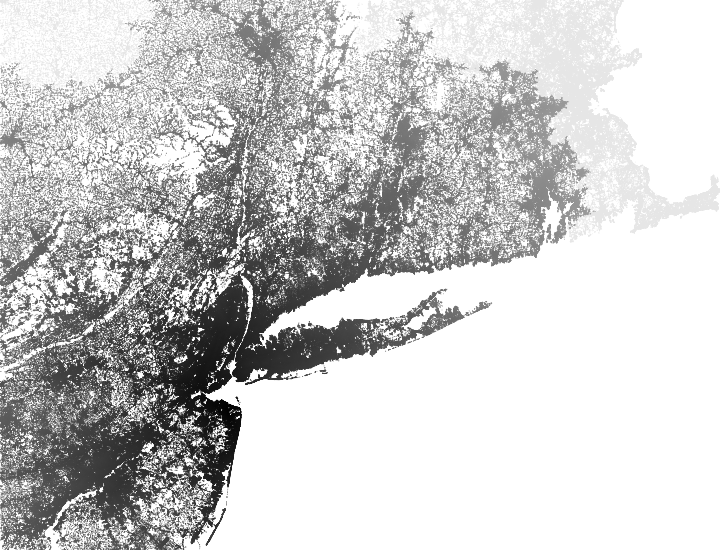
\includegraphics[width=3cm]{figs/incbi-road-ne/singleshot/example-dijkstra.png}};
      \node[draw=black!30,inner sep=0pt] (exdynswsf) at (4.8,3.7) {
         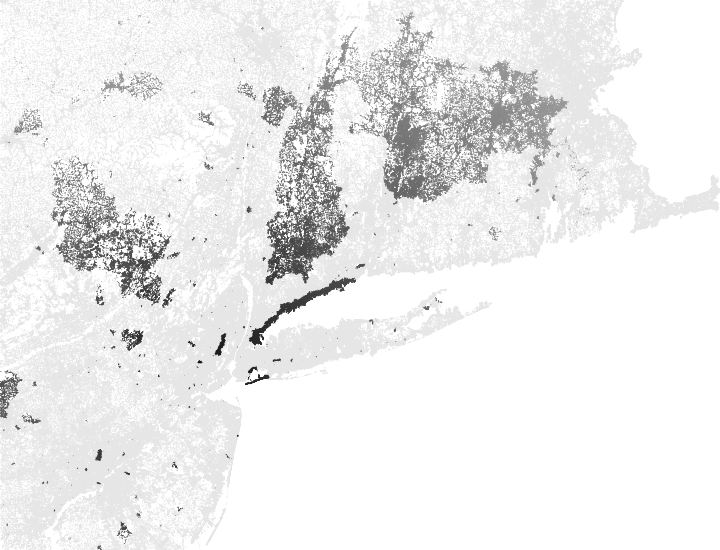
\includegraphics[width=3cm]{figs/incbi-road-ne/singleshot/example-incuni-1.png}};
         
      \node[draw=black!30,inner sep=0pt] (exbidijk) at (1.7,1.3) {
         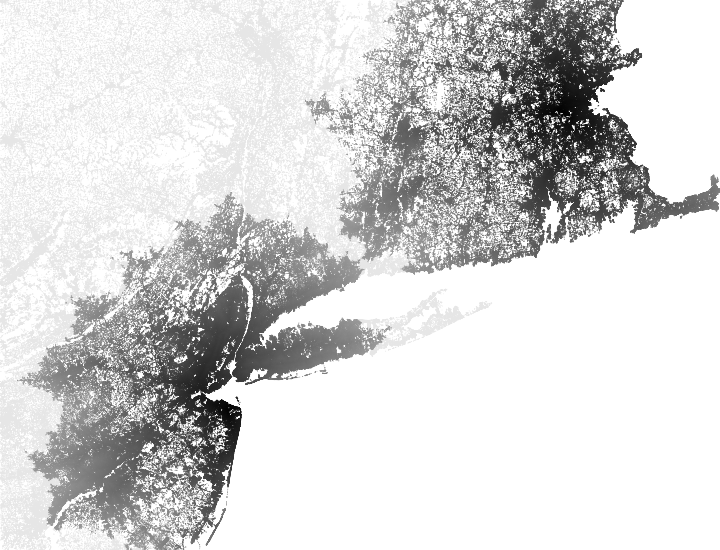
\includegraphics[width=3cm]{figs/incbi-road-ne/singleshot/example-bidijkstra.png}};
      \node[draw=black!30,inner sep=0pt] (exibid) at (4.8,1.3) {
         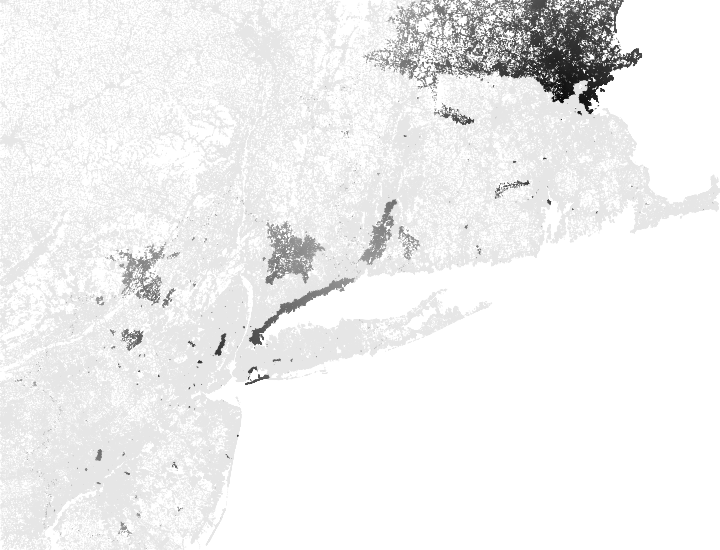
\includegraphics[width=3cm]{figs/incbi-road-ne/singleshot/example-incbi-1.png}};

      \node[anchor=south east] at (exdijk.south east) {Dijk};
      \node[anchor=south east] at (exdynswsf.south east) {DynSWSF};
      \node[anchor=south east] at (exbidijk.south east) {BiDijk};
      \node[anchor=south east] at (exibid.south east) {IBiD};

      \node at (9.2,3.8) {\includegraphics{build/incbi-road-ne/stats2vert-nonheur}};

   \end{tikzpicture}
\end{frame}

\begin{frame}
   \frametitle{Outline of Selected Algorithms}
   \begin{tikzpicture}[font=\small]
      \tikzset{>=latex} % arrow heads
      \draw[step=1,black!15,very thin,opacity=\gridopacity] (0,0) grid (12,8);

      \node[inner sep=0pt,anchor=north] at (6,7.0) {\begin{minipage}{9.05cm}
         \begin{tabular}{ccc}
            \toprule
            & Non-Incremental & Incremental \\
            \midrule
            \addlinespace[0.2em]
            \strut Unidirectional
               & Dijkstra's Algorithm
               & DynamicSWSF-FP \\
            \addlinespace[-0.2em]
            \strut {\only<1>{\color{gray}}\emph{(Heuristic)}}
               & {\only<1>{\color{gray}}\emph{A*}}
               & {\only<1>{\color{gray}}\emph{Lifelong Planning A*}} \\
            \addlinespace[0.3em]
            \strut Bidirectional
               & Bidirectional Dijkstra
               & IBiD \\
            \addlinespace[-0.2em]
            \strut {\only<1>{\color{gray}}\emph{(Heuristic)}}
               & {\only<1>{\color{gray}}\emph{Bidirectional A*}}
               & \only<1>{\color{gray}?}
                 \only<2->{\emph{Heuristic IBiD}} \\
            \addlinespace[0.2em]
            \bottomrule
         \end{tabular}
      \end{minipage}};

      \node[fill=blue!5,draw=blue!15,rounded corners] at (6,4) {\begin{minipage}{10cm}Key Insights:\end{minipage}};

      \node[fill=black!5,draw=black!15,rounded corners,
         anchor=north,minimum width=3.0cm,minimum height=2.5cm] (trustblock) at (2.5,3.6) {};
      \node[fill=white,rounded corners,inner sep=2pt,below=0.1cm of trustblock.north]
         {\includegraphics[height=1.7cm]{build/ibid-dijkstra-trust-build,winctrust}};
      \node[align=center,font=\footnotesize,anchor=south] at (trustblock.south) {Trust Regions};

      \node[fill=black!5,draw=black!15,rounded corners,
         anchor=north,minimum width=3.0cm,minimum height=2.5cm] (termblock) at (6.0,3.6) {};
      \node[fill=white,rounded corners,inner sep=2pt,below=0.1cm of termblock.north]
         {\includegraphics[height=1.5cm]{build/ibid-bidijkstra-viz-build,e}};
      \node[align=center,font=\footnotesize,anchor=south] at (termblock.south) {Bidirectional\\Termination};

      \node[fill=black!5,draw=black!15,rounded corners,
         anchor=north,minimum width=3.0cm,minimum height=2.5cm] (potblock) at (9.5,3.6) {};
      \node[fill=white,rounded corners,inner sep=2pt,below=0.1cm of potblock.north]
         {\includegraphics[height=1.5cm]{build/ibid-potentials}};
      \node[align=center,font=\footnotesize,anchor=south] at (potblock.south) {Potential\\Functions};

      \only<2>{
         \draw[thick,rounded corners] (potblock.south west) rectangle (potblock.north east);
      }

   \end{tikzpicture}
\end{frame}

\begin{frame}
   \frametitle{Heuristics as Vertex Potential Functions}
   \begin{tikzpicture}[font=\small]
   \tikzset{>=latex} % arrow heads
   \draw[step=1,black!15,very thin,opacity=\gridopacity] (0,0) grid (12,8);

   \begin{scope}[shift={(0.2,2.5)}]
   \node at (2.4,4.1) {Directed graph $G = (V,E)$};
   
   % vertices
   \node[fill=black,circle,inner sep=1.3pt] (s) at (1.8,2.0) {};
   \node[fill=black,circle,inner sep=1.3pt] (a) at (2.9,2.9) {};
   \node[fill=black,circle,inner sep=1.3pt] (b) at (3.6,1.2) {};
   \node[fill=black,circle,inner sep=1.3pt] (c) at (2.7,1.7) {};
   \node[fill=black,circle,inner sep=1.3pt] (d) at (1.2,3.6) {};
   \node[fill=black,circle,inner sep=1.3pt] (e) at (1.9,3.1) {};
   \node[fill=black,circle,inner sep=1.3pt] (f) at (3.5,2.0) {}; % frontier
   \node[fill=black,circle,inner sep=1.3pt] (g) at (1.1,2.7) {};
   \node[fill=black,circle,inner sep=1.3pt] (h) at (0.3,3.6) {};
   \node[fill=black,circle,inner sep=1.3pt] (i) at (0.2,2.83) {};
   \node[fill=black,circle,inner sep=1.3pt] (j) at (0.5,2.0) {};
   \node[fill=black,circle,inner sep=1.3pt] (k) at (1.2,1.5) {};
   \node[fill=black,circle,inner sep=1.3pt] (l) at (2.2,1.1) {};
   \node[fill=black,circle,inner sep=1.3pt] (m) at (1.42,0.5) {};
   \node[fill=black,circle,inner sep=1.3pt] (n) at (0.5,0.8) {};
   \node[fill=black,circle,inner sep=1.3pt] (o) at (3.0,0.6) {};
   \node[fill=black,circle,inner sep=1.3pt] (p) at (4.0,0.3) {};
   \node[fill=black,circle,inner sep=1.3pt] (q) at (4.7,0.9) {};
   \node[fill=black,circle,inner sep=1.3pt] (r) at (4.3,1.7) {};
   \node[fill=black,circle,inner sep=1.3pt] (t) at (4.1,2.9) {};
   \node[fill=black,circle,inner sep=1.3pt] (u) at (3.5,3.6) {};
   \node[fill=black,circle,inner sep=1.3pt] (v) at (0.6,0.2) {};

   \draw[->,draw=black!50] (s) -- (c);
   \draw[->,draw=black!50] (s) -- (e);
   \draw[->,draw=black!50] (e) -- (a);
   \draw[->,draw=black!50] (g) -- (e);
   \draw[->,draw=black!50] (e) -- (d);
   \draw[->,draw=black!50] (a) -- (f);
   \draw[->,draw=black!50] (g) -- (j);
   \draw[->,draw=black!50] (g) -- (d);
   \draw[->,draw=black!50] (d) -- (h);
   \draw[->,draw=black!50] (i) -- (h);
   \draw[->,draw=black!50] (g) -- (i);
   \draw[->,draw=black!50] (j) -- (i);
   \draw[->,draw=black!50] (s) -- (g);
   \draw[->,draw=black!50] (k) -- (j);
   \draw[->,draw=black!50] (k) -- (l);
   \draw[->,draw=black!50] (k) -- (n);
   \draw[->,draw=black!50] (j) -- (n);
   \draw[->,draw=black!50] (m) -- (n);
   \draw[->,draw=black!50] (s) -- (j);
   \draw[->,draw=black!50] (s) -- (k);
   \draw[->,draw=black!50] (k) -- (m);
   \draw[->,draw=black!50] (s) -- (l);
   \draw[->,draw=black!50] (l) -- (m);
   \draw[->,draw=black!50] (c) -- (l);
   \draw[->,draw=black!50] (l) -- (o);
   \draw[->,draw=black!50] (o) -- (p);
   \draw[->,draw=black!50] (o) -- (b);
   \draw[->,draw=black!50] (b) -- (p);
   \draw[->,draw=black!50] (b) -- (f);
   \draw[->,draw=black!50] (c) -- (f);
   \draw[->,draw=black!50] (p) -- (q);
   \draw[->,draw=black!50] (b) -- (r);
   \draw[->,draw=black!50] (f) -- (r);
   \draw[->,draw=black!50] (r) -- (q);
   \draw[->,draw=black!50] (f) -- (t);
   \draw[->,draw=black!50] (a) -- (t);
   \draw[->,draw=black!50] (a) -- (u);
   \draw[->,draw=black!50] (u) -- (t);
   \draw[->,draw=black!50] (n) -- (v);
   \end{scope}

   \node[fill=black!3,rounded corners,align=center] (blocka) at (7.3,6.6) {
      \strut $w : E \rightarrow \mathbb{R}$};

   \only<2->{
   \node[fill=black!3,rounded corners,align=center] (blockb) at (7.3,5.5) {
      Vertex potential:\\
      \strut $b : V \rightarrow \mathbb{R}$};
   }

   \only<3->{
   \node[fill=black!3,rounded corners,align=center] (blockc) at (7.3,4.2) {
      \strut $w' : E \rightarrow \mathbb{R}$\\
      \strut $w'_{uv} = w_{uv} - \left( b(u)\!-\!b(v) \right)$};
   }

   \only<4->{
   \node[fill=blue!5,rounded corners,align=center] at (8.5,1.8) {
      $\arraycolsep=1.5pt \begin{array}{rl}
         \vspace{0.1cm}
         \mbox{len}(p_{st}, w') = & w'_{su} + w'_{uv} \dots \\
          = & w_{su} - \left( b(s)\!-\!b(u) \right) \\
          & + \; w_{su} - \left( b(u)\!-\!b(v) \right) \\
          & + \; \dots \vspace{0.1cm} \\
          = & \mbox{len}(p_{st}, w) - \left( b(s)\!-\!b(t) \right)
      \end{array}$\\
      \vspace{0.0cm}\\
      Length difference independent of $p_{st}$!};
   }

   \only<5->{
   \node[fill=blue!5,rounded corners,align=center] (blockd) at (10.7,4.2) {
      Shortest path\\ \strut $p'_{st}$ w.r.t. $w'$};
   }

   \only<6->{
   \node[fill=blue!5,rounded corners,align=center] (blocke) at (10.7,6.6) {
      Shortest path\\ \strut $p_{st}$ w.r.t. $w$};
   }

   \only<7->{\draw[->] (blocka) -- (blockb);}
   \only<8->{\draw[->] (blockb) -- (blockc);}
   \only<9->{\draw[->] (blockc) -- (blockd);}
   \only<10->{\draw[->] (blockd) -- (blocke);}
   

   \end{tikzpicture}
\end{frame}

\begin{frame}
   \frametitle{Heuristics as Vertex Potential Functions}
   \begin{tikzpicture}[font=\small]
   \tikzset{>=latex} % arrow heads
   \draw[step=1,black!15,very thin,opacity=\gridopacity] (0,0) grid (12,8);

   \node[fill=black!3,minimum width=5.2cm] at (3.7,7.55) {\strut Non-Incremental};
   \node[fill=black!3,minimum width=3.3cm,rotate=90] at (0.6,5.45) {\strut Unidirectional};
   \only<6->{\node[fill=black!3,minimum width=5.2cm] at (9.0,7.55) {\strut Incremental};}
   \only<17->{\node[fill=black!3,minimum width=3.45cm,rotate=90] at (0.6,1.85) {\strut Bidirectional};}

   \only<2->{
   \node[fill=blue!5,rounded corners,anchor=north,minimum width=5cm,minimum height=3.3cm] (dijk) at (3.7,7.1) {};
   \node[anchor=north] at (dijk.north) {\begin{minipage}{4.7cm}
      \setlength{\belowdisplayskip}{1pt} \setlength{\belowdisplayshortskip}{1pt}
      \setlength{\abovedisplayskip}{1pt} \setlength{\abovedisplayshortskip}{1pt}

      Use potential function:
      \[
         b(v) = h_t(v)
      \]
      \[
         w'_{uv} = w_{uv} - \left( b(u)\!-\!b(v) \right) 
      \]
      
      \only<5->{
      \vspace{0.7cm}
      \begin{center}
         Dijkstra's algorithm on $w'$\\
         yields A*
      \end{center}}
   \end{minipage}};
   }
   \only<3->{\node[fill=blue!10,rounded corners,inner sep=3pt,align=center] (dijkin) at (2.7,5.2) {$w \geq 0$\\$h_t$ consistent};}
   \only<4->{
      \node[fill=blue!10,rounded corners,inner sep=3pt] (dijkout) at (5.2,5.2) {$w_{uv}' \geq 0$};
      \draw[->] (dijkin) -- (dijkout);}


   \only<7->{
   \node[fill=blue!5,rounded corners,anchor=north,minimum width=5cm,minimum height=3.3cm] (dynswsffp) at (9.0,7.1) {};
   \only<24->{
      \node[fill=green!20,anchor=north,minimum width=5cm,minimum height=0.55cm,below=0.85cm of dynswsffp.north]  {};
   }
   \node[anchor=north] at (dynswsffp.north) {\begin{minipage}{4.7cm}
      \setlength{\belowdisplayskip}{1pt} \setlength{\belowdisplayshortskip}{1pt}
      \setlength{\abovedisplayskip}{1pt} \setlength{\abovedisplayshortskip}{1pt}
      \only<8->{
      Use potential function:
      \[
         b(v) = h_t(v)
      \]}%
      \only<9-11>{\[
         w'_{uv} = w_{uv} - \left( b(u)\!-\!b(v) \right)
      \]}%
      \only<13-15>{\[
         w'_{uv} = \left[ w_{uv} - \left( b(u)\!-\!b(v) \right), \;\;\, ? \;\;\; \right]
      \]}%
      \only<16->{\[
         w'_{uv} = \left[ w_{uv} - \left( b(u)\!-\!b(v) \right), \; w_{uv} \right]
      \]}%
      
      \only<15->{%
      \vspace{0.7cm}
      \begin{center}
         DynamicSWSF-FP on $w'$\\
         yields LPA*
      \end{center}%
      }
   \end{minipage}};
   }
   \only<10->{\node[fill=blue!10,rounded corners,inner sep=3pt,align=center] (dynswsffpin) at (8.0,5.2) {$w_{uv} > 0$\\$h_t$ consistent};}
   \only<11>{
      \node[fill=blue!10,rounded corners,inner sep=3pt] (dynswsffpout) at (10.5,5.2) {$w_{uv}' \ngtr 0$};
      \draw[->] (dynswsffpin) -- (dynswsffpout);}
   \only<14->{
      \node[fill=blue!10,rounded corners,inner sep=3pt] (dynswsffpout) at (10.5,5.2) {$w_{uv}' > [0,0]$};
      \draw[->] (dynswsffpin) -- (dynswsffpout);}


   \only<18->{
   \node[fill=blue!5,rounded corners,anchor=north,minimum width=5cm,minimum height=3.5cm] (bidijk) at (3.7,3.6) {};
   \only<22->{
      \node[fill=green!20,anchor=north,minimum width=5cm,minimum height=0.55cm,below=0.45cm of bidijk.north]  {};
   }
   \node[anchor=north] at (bidijk.north) {\begin{minipage}{4.7cm}
      \setlength{\belowdisplayskip}{2pt} \setlength{\belowdisplayshortskip}{2pt}
      \setlength{\abovedisplayskip}{2pt} \setlength{\abovedisplayshortskip}{2pt}

      Use potential function:
      \[
         b(v) = \tfrac{1}{2} h_t(v) - \tfrac{1}{2} h_s(v)
      \]
      \[
         w'_{uv} = w_{uv} - \left( b(u)\!-\!b(v) \right) 
      \]

      \vspace{0.7cm}
      \begin{center}
         Bidirectional Dijkstra's on $w'$\\
         yields Bidirectional A*
      \end{center}
   \end{minipage}};
   }
   \only<18>{
      \node[fill=blue!5,anchor=north,rounded corners,minimum width=5cm,minimum height=1.0cm,below=0.0cm of bidijk.north] {};
   }
   \only<18-19>{
      \node[fill=blue!10,rounded corners,inner sep=3pt,align=center] (bidijkin) at (2.7,1.6) {$w \geq 0$\\ \strut $b$ consistent};
   }
   \only<20->{
      \node[fill=blue!10,rounded corners,inner sep=3pt,align=center] (bidijkin) at (2.7,1.6) {$w \geq 0$\\ \strut $h_s, h_t$ consistent};
   }
   \only<18->{
      \node[fill=blue!10,rounded corners,inner sep=3pt] (bidijkout) at (5.2,1.6) {$w' \geq 0$};
      \draw[->] (bidijkin) -- (bidijkout);
   }


   \only<21->{
   \node[fill=blue!5,rounded corners,anchor=north,minimum width=5cm,minimum height=3.5cm] (ibid) at (9.0,3.6) {};
   \only<23-24>{
      \node[fill=green!20,anchor=north,minimum width=5cm,minimum height=0.55cm,below=0.45cm of ibid.north]  {};
   }
   \only<25->{
      \node[fill=green!20,anchor=north,minimum width=5cm,minimum height=1.05cm,below=0.45cm of ibid.north]  {};
   }
   \node[anchor=north] at (ibid.north) {\begin{minipage}{4.7cm}
      \setlength{\belowdisplayskip}{2pt} \setlength{\belowdisplayshortskip}{2pt}
      \setlength{\abovedisplayskip}{2pt} \setlength{\abovedisplayshortskip}{2pt}
      \only<23->{
      Use potential function:
      \[
         b(v) = \tfrac{1}{2} h_t(v) - \tfrac{1}{2} h_s(v)
      \]}%
      \only<25->{\[
         w'_{uv} = \left[ w_{uv} - \left( b(u)\!-\!b(v) \right), \; w_{uv} \right]
      \]}%
      \only<26->{%
      \vspace{0.38cm}
      \begin{center}
         IBiD on $w'$\\
         yields Heuristic IBiD
      \end{center}
      }
   \end{minipage}};
   }
   \only<26->{
   \node[fill=blue!10,rounded corners,inner sep=3pt,align=center] (ibidin) at (8.0,1.6) {$w_{uv} > 0$\\$h_s, h_t$ consistent};
   \node[fill=blue!10,rounded corners,inner sep=3pt] (ibidout) at (10.5,1.6) {$w_{uv}' > [0,0]$};
   \draw[->] (ibidin) -- (ibidout);
   }
   

   \end{tikzpicture}
\end{frame}

\begin{frame}
   \frametitle{Traffic Problem Results: With Euclidean Heuristic}
   \begin{tikzpicture}[font=\small]
      \tikzset{>=latex} % arrow heads
      \draw[step=1,black!15,very thin,opacity=\gridopacity] (0,0) grid (12,8);

      \node at (6,3.8) {\includegraphics{build/incbi-road-ne/stats2vert}};

   \end{tikzpicture}
\end{frame}

\begin{frame}
   \frametitle{Experiment: Traffic Problem}
   \begin{tikzpicture}[font=\small]
      \draw[step=1,black!15,very thin,opacity=\gridopacity] (0,0) grid (12,8);
      
      \node[inner sep=0pt] (vidnode) at (6,4.0) {%
         \href{\tikzvidtarget{incbi-roadne}}{%
         \includegraphics[width=11cm]{videos/incbi-roadne.png}}};
      \tikzvidplayat{incbi-roadne}{vidnode}{videos/incbi-roadne.mp4}{}

   \end{tikzpicture}
\end{frame}

\begin{frame}
   \frametitle{LazySP Problem: Dynamic SP Algorithms}
   \begin{tikzpicture}[font=\small]
      \draw[step=1,black!15,very thin,opacity=\gridopacity] (0,0) grid (12,8);

      \node at (6,4) {\includegraphics{build/ibid-lazysp-plot}};

      %\node[draw=black,inner sep=0pt,thick] at (5.35,6.235) {\includegraphics[width=2.0cm]{figs/herbarm-traj2-t031.png}};
      \node[draw=black,inner sep=0pt,thick,anchor=north] at (5.15,7.325) {\includegraphics[width=2.0cm]{figs/herbarm-traj2-t031.png}};
      \node[draw=black,fill=black!2,anchor=north] at (7.8,7.325) {\strut $h_w = (1 - \lambda) \, h_x$};

   \end{tikzpicture}
\end{frame}


\begin{frame}
   \frametitle{Outline of Selected Algorithms}
   \begin{tikzpicture}[font=\small]
      \tikzset{>=latex} % arrow heads
      \draw[step=1,black!15,very thin,opacity=\gridopacity] (0,0) grid (12,8);

      \node[inner sep=0pt,anchor=north] at (6,7.0) {\begin{minipage}{9.05cm}
         \begin{tabular}{ccc}
            \toprule
            & Non-Incremental & Incremental \\
            \midrule
            \addlinespace[0.2em]
            \strut Unidirectional
               & Dijkstra's Algorithm
               & DynamicSWSF-FP \\
            \addlinespace[-0.2em]
            \strut \emph{(Heuristic)}
               & \emph{A*}
               & \emph{Lifelong Planning A*} \\
            \addlinespace[0.3em]
            \strut Bidirectional
               & Bidirectional Dijkstra
               & IBiD \\
            \addlinespace[-0.2em]
            \strut \emph{(Heuristic)}
               & \emph{Bidirectional A*}
               & \emph{Heuristic IBiD} \\
            \addlinespace[0.2em]
            \bottomrule
         \end{tabular}
      \end{minipage}};

      \node[fill=blue!5,draw=blue!15,rounded corners] at (6,4) {\begin{minipage}{10cm}Key Insights:\end{minipage}};

      \node[fill=black!5,draw=black!15,rounded corners,
         anchor=north,minimum width=3.0cm,minimum height=2.5cm] (trustblock) at (2.5,3.6) {};
      \node[fill=white,rounded corners,inner sep=2pt,below=0.1cm of trustblock.north]
         {\includegraphics[height=1.7cm]{build/ibid-dijkstra-trust-build,winctrust}};
      \node[align=center,font=\footnotesize,anchor=south] at (trustblock.south) {Trust Regions};

      \node[fill=black!5,draw=black!15,rounded corners,
         anchor=north,minimum width=3.0cm,minimum height=2.5cm] (termblock) at (6.0,3.6) {};
      \node[fill=white,rounded corners,inner sep=2pt,below=0.1cm of termblock.north]
         {\includegraphics[height=1.5cm]{build/ibid-bidijkstra-viz-build,e}};
      \node[align=center,font=\footnotesize,anchor=south] at (termblock.south) {Bidirectional\\Termination};

      \node[fill=black!5,draw=black!15,rounded corners,
         anchor=north,minimum width=3.0cm,minimum height=2.5cm] (potblock) at (9.5,3.6) {};
      \node[fill=white,rounded corners,inner sep=2pt,below=0.1cm of potblock.north]
         {\includegraphics[height=1.5cm]{build/ibid-potentials}};
      \node[align=center,font=\footnotesize,anchor=south] at (potblock.south) {Potential\\Functions};

   \end{tikzpicture}
\end{frame}
